\let\negmedspace\undefined
\let\negthickspace\undefined
\documentclass[journal,12pt,onecolumn]{IEEEtran}
\usepackage{cite}
\usepackage{amsmath,amssymb,amsfonts,amsthm}
\usepackage{algorithmic}
\usepackage{graphicx}
\graphicspath{{./figs/}}
\usepackage{textcomp}
\usepackage{xcolor}
\usepackage{txfonts}
\usepackage{listings}
\usepackage{enumitem}
\usepackage{mathtools}
\usepackage{gensymb}
\usepackage{comment}
\usepackage{caption}
\usepackage[breaklinks=true]{hyperref}
\usepackage{tkz-euclide} 
\usepackage{listings}
\usepackage{gvv}                                        
%\def\inputGnumericTable{}                                 
\usepackage[latin1]{inputenc}     
\usepackage{xparse}
\usepackage{color}                                            
\usepackage{array}                                            
\usepackage{longtable}                                       
\usepackage{calc}                                             
\usepackage{multirow}
\usepackage{multicol}
\usepackage{hhline}                                           
\usepackage{ifthen}                                           
\usepackage{lscape}
\usepackage{tabularx}
\usepackage{array}
\usepackage{float}
\newtheorem{theorem}{Theorem}[section]
\newtheorem{problem}{Problem}
\newtheorem{proposition}{Proposition}[section]
\newtheorem{lemma}{Lemma}[section]
\newtheorem{corollary}[theorem]{Corollary}
\newtheorem{example}{Example}[section]
\newtheorem{definition}[problem]{Definition}
\newcommand{\BEQA}{\begin{eqnarray}}
\newcommand{\EEQA}{\end{eqnarray}}
\newcommand{\define}{\stackrel{\triangle}{=}}
\theoremstyle{remark}
\newtheorem{rem}{Remark}


\begin{document}

\title{
Assignment : GATE 2014 MA}
\author{EE25BTECH11061 - Vankudoth Sainadh}
\maketitle
\renewcommand{\thefigure}{\theenumi}
\renewcommand{\thetable}{\theenumi}

\begin{enumerate}

\item A student is required to demonstrate a high level of \underline{\text{comprehension}} of the subject, especially in the social sciences.\\
The word closest in meaning to \underline{\text{comprehension}} is 

\hfill{\brak{\text{{GATE MA 2014}}}

\begin{enumerate}
\begin{multicols}{4}
\item understanding
\item meaning
\item concentration
\item stability
\end{multicols}
\end{enumerate}

\item Choose the most appropriate word from the options given below to complete the following sentence.\\
One of his biggest \underline{\hspace{2cm}} was his ability to forgive. 

\hfill{\brak{\text{{GATE MA 2014}}}

\begin{enumerate}
\begin{multicols}{4}
\item vice
\item virtues
\item choices
\item strength
\end{multicols}
\end{enumerate}

\item Rajan was not happy that Sajan decided to do the project on his own. On observing his unhappiness, Sajan explained to Rajan that he preferred to work independently.\\
Which one of the statements below is logically valid and can be inferred from the above sentences?

\hfill{\brak{\text{{GATE MA 2014}}}}

\begin{enumerate}
\item Rajan has decided to work only in a group.
\item Rajan and Sajan were formed into a group against their wishes.
\item Sajan had decided to give in to Rajan's request to work with him.
\item Rajan had believed that Sajan and he would be working together.
\end{enumerate}

\item If $y=5x^{2}+3$, then the tangent at $x=0,\ y=3$ 

\hfill{\brak{\text{GATE MA 2014}}}

\begin{enumerate}
\begin{multicols}{2}
\item passes through $x=0,\ y=0$
\item has a slope of $+1$
\item is parallel to the $x$-axis
\item has a slope of $-1$
\end{multicols}
\end{enumerate}

\item A foundry has a fixed daily cost of Rs $50{,}000$ whenever it operates and a variable cost of Rs $800Q$, where $Q$ is the daily production in tonnes. What is the cost of production in Rs per tonne for a daily production of $100$ tonnes?

\hfill{\brak{\text{GATE MA 2014}}}

\item Find the odd one in the following group: \texttt{ALRVX}, \texttt{EPVZB}, \texttt{ITZDF}, \texttt{OYEIK} \hfill{\brak{\text{GATE MA 2014}}}
\begin{enumerate}
\begin{multicols}{4}
\item ALRVX
\item EPVZB
\item ITZDF
\item OYEIK
\end{multicols}
\end{enumerate}

\item Anuj, Bhola, Chandan, Dilip, Eswar and Faisal live on different floors in a six-storeyed building (the ground floor is numbered $1$, the floor above it $2$, and so on). Anuj lives on an even-numbered floor. Bhola does not live on an odd numbered floor. Chandan does not live on any of the floors below Faisal's floor. Dilip does not live on floor number $2$. Eswar does not live on a floor immediately above or immediately below Bhola. Faisal lives three floors above Dilip. Which of the following floor-person combinations is correct? 

\hfill{\brak{\text{GATE MA 2014}}}

\begin{center}
\renewcommand{\arraystretch}{1.2}
\begin{tabular}{|c|c|c|c|c|c|c|}
\hline
 & Anuj & Bhola & Chandan & Dilip & Eswar & Faisal\\
\hline
(A) & 6 & 2 & 5 & 1 & 3 & 4\\
\hline
(B) & 2 & 6 & 5 & 1 & 3 & 4\\
\hline
(C) & 4 & 2 & 6 & 3 & 1 & 5\\
\hline
(D) & 2 & 4 & 6 & 1 & 3 & 5\\
\hline
\end{tabular}
\end{center}

\item The smallest angle of a triangle is equal to two-thirds of the smallest angle of a quadrilateral. The ratio between the angles of the quadrilateral is $3:4:5:6$. The largest angle of the triangle is twice its smallest angle. What is the sum, in degrees, of the second largest angle of the triangle and the largest angle of the quadrilateral?

\hfill{\brak{\text{GATE MA 2014}}}

\item One percent of the people of country $X$ are taller than $6$ ft. Two percent of the people of country $Y$ are taller than $6$ ft. There are thrice as many people in country $X$ as in country $Y$. Taking both countries together, what is the percentage of people taller than $6$ ft? 

\hfill{\brak{\text{GATE MA 2014}}}

\begin{enumerate}
\begin{multicols}{4}
\item 3.0
\item 2.5
\item 1.5
\item 1.25
\end{multicols}
\end{enumerate}

\item The monthly rainfall chart based on $50$ years of rainfall in Agra is shown in the following figure. Which of the following are true? \brak{k} percentile is the value such that k percent of the data fall below that value}

\hfill{\brak{\text{GATE MA 2014}}}

\begin{figure}[h!]
\centering
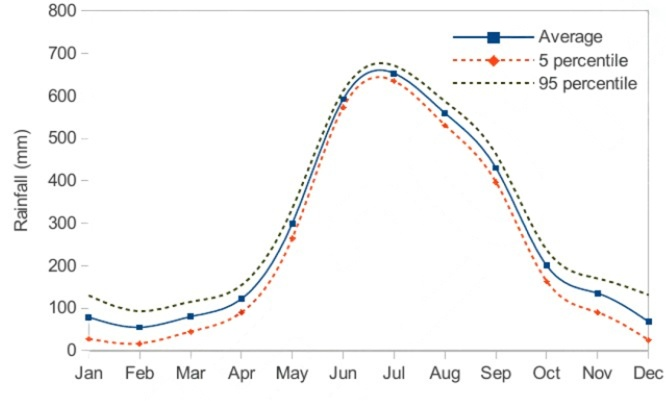
\includegraphics[width=.85\linewidth]{figs/FIG1.png}
\caption{*}
\label{fig:placeholder}
\end{figure}

\begin{enumerate}
\item On average, it rains more in July than in December
\item Every year, the amount of rainfall in August is more than that in January
\item July rainfall can be estimated with better confidence than February rainfall
\item In August, there is at least $500$ mm of rainfall
\end{enumerate}

\begin{enumerate}
\begin{multicols}{2}
\item (i) and (ii)
\item (i) and (iii)
\item (ii) and (iii)
\item (iii) and (iv)
\end{multicols}
\end{enumerate}


\item The function $f(z)=\bar z^{\,2}+i\,\bar z+1$ is differentiable at

\hfill{\brak{\text{GATE MA 2014}}}

\begin{enumerate}
\begin{multicols}{4}
\item $i$
\item $1$
\item $-i$
\item no point in $\mathbb{C}$
\end{multicols}
\end{enumerate}


\item The radius of convergence of the power series
\begin{align*}
\sum_{n=0}^{\infty} 4^{\,(-1)^{n} n}\, z^{2n}
\end{align*}
is \underline{\hspace{2.5cm}}.

\hfill{\brak{\text{GATE MA 2014}}}

\item Let $E_1$ and $E_2$ be two non empty subsets of a normed linear space $X$, and let
\begin{align*}
E_{1}+E_{2}\;:=\;\{\,x+y\in X : x\in E_{1}\ \text{and}\ y\in E_{2}\,\}.
\end{align*}
Which of the following statements is \textbf{FALSE}?

\hfill{\brak{\text{GATE MA 2014}}}

\begin{enumerate}
\item If $E_1$ and $E_2$ are convex, then $E_1+E_2$ is convex
\item If either $E_1$ or $E_2$ is open, then $E_1+E_2$ is open
\item $E_1+E_2$ must be closed if $E_1$ and $E_2$ are closed
\item If $E_1$ is closed and $E_2$ is compact, then $E_1+E_2$ is closed
\end{enumerate}


\item Let $y(x)$ be the solution to the initial value problem
\begin{align*}
\frac{dy}{dx}=\sqrt{y}+2x, \qquad y(1.2)=2.
\end{align*}
Using the Euler method with step size $h=0.05$, the approximate value of $y(1.3)$,
correct to two decimal places, is \underline{\hspace{3cm}}.

\hfill{\brak{\text{GATE MA 2014}}}

\item Let $\alpha\in\mathbb{R}$. If $\alpha x$ is the polynomial which
interpolates the function $f(x)=\sin(\pi x)$ on $[-1,1]$ at all the zeroes
of the polynomial $4x^{3}-3x$, then $\alpha$ is
\underline{\hspace{2.0cm}}.

\hfill{\brak{\text{GATE MA 2014}}}

\item If $u(x,t)$ is the D'Alembert's solution to the wave equation
\begin{align*}
\frac{\partial^{2}u}{\partial t^{2}}=\frac{\partial^{2}u}{\partial x^{2}},
\qquad x\in\mathbb{R},\ t>0,
\end{align*}
with the conditions $u(x,0)=0$ and $\dfrac{\partial u}{\partial t}(x,0)=\cos x$,
then $u\!\left(0,\dfrac{\pi}{4}\right)$ is \underline{\hspace{2.2cm}}.

\hfill{\brak{\text{GATE MA 2014}}}

\item The solution of the integral equation
\begin{align*}
\phi(x)=x+\int_{0}^{x}\sin(x-\xi)\,\phi(\xi)\,d\xi
\end{align*}
is
\hfill{\brak{\text{GATE MA 2014}}}

\begin{enumerate}
\begin{multicols}{4}
\item $x^{2}+\dfrac{x^{3}}{3}$
\item $x-\dfrac{x^{3}}{3!}$
\item $x+\dfrac{x^{3}}{3!}$
\item $x^{2}-\dfrac{x^{3}}{3!}$
\end{multicols}
\end{enumerate}
\newpage

\item The general solution to the ordinary differential equation
\begin{align*}
x^{2}\frac{d^{2}y}{dx^{2}}+x\frac{dy}{dx}+\left(4x^{2}-\frac{9}{25}\right)y=0
\end{align*}
in terms of Bessel's functions $J_\nu(\cdot)$, is
\nolinebreak

\hfill\mbox{\brak{\text{GATE MA 2014}}}

\begin{enumerate}
\begin{multicols}{2}
\item $y(x)=c_{1}\,J_{3/5}(2x)+c_{2}\,J_{-3/5}(2x)$
\item $y(x)=c_{1}\,J_{3/10}(x)+c_{2}\,J_{-3/10}(x)$
\item $y(x)=c_{1}\,J_{3/5}(x)+c_{2}\,J_{-3/5}(x)$
\item $y(x)=c_{1}\,J_{3/10}(2x)+c_{2}\,J_{-3/10}(2x)$
\end{multicols}
\end{enumerate}

\item The inverse Laplace transform of
\begin{align*}
\frac{2s^{2}-4}{(s-3)\,(s^{2}-s-2)}
\end{align*}
is
\makebox[\linewidth][r]{\brak{\text{GATE MA 2014}}}

\begin{enumerate}
\begin{multicols}{2}
\item $(1+t)\,e^{-t}+\dfrac{7}{2}\,e^{-3t}$
\item \(\dfrac{e^{t}}{3}+t\,e^{-t}+2t\)
\item \(\dfrac{7}{2}\,e^{3t}-\dfrac{e^{-t}}{6}-\dfrac{4}{3}\,e^{2t}\)
\item \(\dfrac{7}{2}\,e^{-3t}-\dfrac{e^{t}}{6}-\dfrac{4}{3}\,e^{-2t}\)
\end{multicols}
\end{enumerate}


\item If $X_1,X_2$ is a random sample of size $2$ from $\mathcal{N}(0,1)$ population, then
\begin{align*}
\frac{(X_1+X_2)^{2}}{(X_1-X_2)^{2}}\ \text{follows}
\end{align*} follows

\hfill{\brak{\text{GATE MA 2014}}}

\begin{enumerate}
\begin{multicols}{2}
\item $\chi^{2}(2)$
\item $F(2,2)$
\item $F(2,1)$
\item $F(1,1)$
\end{multicols}
\end{enumerate}


\item Let $Z\sim\mathcal{N}(0,1)$ be a random variable. Then the value of $\mathbb{E}\!\left[\max\{Z,0\}\right]$ is

\makebox[\linewidth][r]{\brak{\text{GATE MA 2014}}}

\begin{enumerate}
\begin{multicols}{4}
\item $\dfrac{1}{\sqrt{\pi}}$
\item $\sqrt{\dfrac{2}{\pi}}$
\item $\dfrac{1}{\sqrt{2\pi}}$
\item $\dfrac{1}{\pi}$
\end{multicols}
\end{enumerate}

\item The number of non-isomorphic groups of order $10$ is
\underline{\hspace{2.5cm}}.

\hfill{\brak{\text{GATE MA 2014}}}

\item Let $a,b,c,d\in\mathbb{R}$ with $a<c<d<b$. Consider the ring $C[a,b]$ with
pointwise addition and multiplication. If
\begin{align*}
S=\{\,f\in C[a,b]: f(x)=0 \text{ for all } x\in[c,d]\,\},
\end{align*}
then

\makebox[\linewidth][r]{\brak{\text{GATE MA 2014}}}

\begin{enumerate}
\begin{multicols}{2}
\item $S$ is NOT an ideal of $C[a,b]$
\item $S$ is an ideal of $C[a,b]$ but NOT a prime ideal of $C[a,b]$
\item $S$ is a prime ideal of $C[a,b]$ but NOT a maximal ideal of $C[a,b]$
\item $S$ is a maximal ideal of $C[a,b]$
\end{multicols}
\end{enumerate}
\newpage
\item Let $R$ be a ring. If $R[x]$ is a principal ideal domain, then $R$ is necessarily a

\hfill{\brak{\text{GATE MA 2014}}}

\begin{enumerate}
\begin{multicols}{2}
\item Unique Factorization Domain
\item Principal Ideal Domain
\item Euclidean Domain
\item Field
\end{multicols}
\end{enumerate}

\item Consider the group homomorphism $\varphi:M_{2}(\mathbb{R})\to\mathbb{R}$ given by
$\varphi(A)=\operatorname{trace}(A)$. The kernel of $\varphi$ is isomorphic to

\hfill{\brak{\text{GATE MA 2014}}}

\begin{enumerate}
\begin{multicols}{2}
\item $\{A\in M_{2}(\mathbb{R}) : \varphi(A)=0\}$
\item $\mathbb{R}^{2}$
\item $\mathbb{R}^{3}$
\item $\mathrm{GL}_{2}(\mathbb{R})$
\end{multicols}
\end{enumerate}

\item  Let $X$ be a set with at least two elements. Let $\tau$ and $\tau'$ be two
topologies on $X$ with $\tau'\ne\{\varnothing,X\}$. Which of the following
conditions is necessary for the identity function
$\mathrm{id}:(X,\tau)\to (X,\tau')$ to be continuous?

\makebox[\linewidth][r]{\textit{(GATE MA 2014)}}

\begin{enumerate}
\begin{multicols}{2}
\item $\tau\subseteq\tau'$
\item $\tau'\subseteq\tau$
\item no conditions on $\tau$ and $\tau'$
\item $\tau\cap\tau'=\{\varnothing,X\}$
\end{multicols}
\end{enumerate}

\item Let $A\in M_{3}(\mathbb{R})$ satisfy $\det(A-I)=0$. If $\operatorname{trace}(A)=13$ and
$\det(A)=32$, then the sum of squares of the eigenvalues of $A$ is
\underline{\hspace{2.5cm}}.

\hfill{\brak{\text{GATE MA 2014}}}

\item Consider the group homomorphism \(\varphi:M_{2}(\mathbb{R})\to\mathbb{R}\) given by
\(\varphi(A)=\operatorname{trace}(A)\). The kernel of \(\varphi\) is isomorphic to which of the
following groups?
\makebox[\linewidth][r]{(GATE MA 2014)}

\begin{enumerate}
\begin{multicols}{2}
\item \( M_{2}(\mathbb{R}) \big/ \{\,A\in M_{2}(\mathbb{R}) : \varphi(A)=0\,\} \)
\item \( \mathbb{R}^{2} \)
\item \( \mathbb{R}^{3} \)
\item \( \mathrm{GL}_{2}(\mathbb{R}) \)
\end{multicols}
\end{enumerate}

\item Let $V$ be a real inner product space of dimension $10$.
Let $x,y\in V$ be non-zero vectors such that $\langle x,y\rangle=0$.
Then the dimension of $\{x\}^{1}\cap\{y\}^{1}$ is \underline{\hspace{3cm}}.

\hfill{\brak{\text{GATE MA 2014}}}

\item Consider the following linear programming problem\\
Minimize\quad $x_1+x_2$\\
Subject to

\begin{align*}
2x_1+x_2\ge 8,\qquad 2x_1+5x_2\ge 10,\qquad x_1,x_2\ge 0.
\end{align*}

The optimal value to this problem is \underline{\hspace{3.2cm}}.

\hfill{\brak{\text{GATE MA 2014}}}

\item Let

\begin{align*}
f(x)=
\begin{cases}
-3\pi, & -\pi<x\le 0,\\[2pt]
\ \,3\pi, & 0<x<\pi,
\end{cases}
\qquad\text{and extend $f$ to be $2\pi$-periodic.}
\end{align*}

The coefficient of $\sin(3x)$ in the Fourier series expansion of $f(x)$ on
$[-\pi,\pi]$ is \underline{\hspace{3.0cm}}.

\makebox[\linewidth][r]{\textit{(GATE MA 2014)}}
\newpage
\item For the sequence of functions

\begin{align*}
f_n(x)=\frac{1}{x^{2}}\sin\!\left(\frac{1}{n x}\right),\qquad x\in[1,\infty),
\end{align*}
consider the following quantities expressed in terms of Lebesgue integrals:
\begin{align*}
\text{I}:\ \lim_{n\to\infty}\int_{1}^{\infty} f_n(x)\,dx,
\qquad
\text{II}:\ \int_{1}^{\infty}\Bigl(\lim_{n\to\infty} f_n(x)\Bigr)\,dx.
\end{align*}
Which of the following is \textbf{TRUE}?

\makebox[\linewidth][r]{\textit{(GATE MA 2014)}}

\begin{enumerate}
\item The limit in I does not exist
\item The integrand in II is not integrable on $[1,\infty)$
\item Quantities I and II are well-defined, but I $\ne$ II
\item Quantities I and II are well-defined and I $=$ II
\end{enumerate}


\item  Which of the following statements about the spaces $\ell^{p}$ and $L^{p}[0,1]$ is \textbf{TRUE}?

\hfill{\brak{\text{GATE MA 2014}}}

\begin{enumerate}
\begin{multicols}{2}
\item $\ell^{3}\subset \ell^{7}$ \ \text{and}\  $L^{6}[0,1]\subset L^{9}[0,1]$
\item $\ell^{3}\subset \ell^{7}$ \ \text{and}\  $L^{9}[0,1]\subset L^{6}[0,1]$
\item $\ell^{7}\subset \ell^{3}$ \ \text{and}\  $L^{6}[0,1]\subset L^{9}[0,1]$
\item $\ell^{7}\subset \ell^{3}$ \ \text{and}\  $L^{9}[0,1]\subset L^{6}[0,1]$
\end{multicols}
\end{enumerate}


\item The maximum modulus of $e^{z^{2}}$ on the set
\begin{align*}
S=\{\, z\in\mathbb{C} : 0\le \Re(z)\le 1,\; 0\le \Im(z)\le 1 \,\}
\end{align*}
is
\hfill{\brak{\text{GATE MA 2014}}}

\begin{enumerate}
\begin{multicols}{4}
\item $2/e$
\item $e$
\item $e+1$
\item $e^{2}$
\end{multicols}
\end{enumerate}

\item Let $d_1,\,d_2$ and $d_3$ be metrics on a set $X$ with at least two elements.
Which of the following is \emph{NOT} a metric on $X$?

\hfill{\brak{\text{GATE MA 2014}}}

\begin{enumerate}
\begin{multicols}{2}
\item $\min\{d_1,\,2\}$
\item $\max\{d_2,\,2\}$
\item $\displaystyle \frac{d_3}{\,1+d_3\,}$
\item $\displaystyle \frac{d_1+d_2+d_3}{3}$
\end{multicols}
\end{enumerate}

\item Let $\Omega=\{\,z\in\mathbb{C}:\Im(z)>0\,\}$ and let $C$ be a smooth curve
lying in $\Omega$ with initial point $-1+2i$ and final point $1+2i$.  
The value of $\displaystyle \int_{C}\frac{1+2z}{1+z}\,dz$ is

\hfill{\brak{\text{GATE MA 2014}}}

\begin{enumerate}
\begin{multicols}{2}
\item $4-\dfrac{1}{2}\ln 2\;+\;i\,\dfrac{\pi}{4}$
\item $-\,4+\dfrac{1}{2}\ln 2\;+\;i\,\dfrac{\pi}{4}$
\item $4+\dfrac{1}{2}\ln 2\;-\;i\,\dfrac{\pi}{4}$
\item $4-\dfrac{1}{2}\ln 2\;+\;i\,\dfrac{\pi}{2}$
\end{multicols}
\end{enumerate}

\item If $a\in\mathbb{C}$ with $|a|<1$, then the value of
\begin{align*}
\frac{1-|a|^{2}}{\pi}\int_{\Gamma}\frac{|dz|}{\,|\,z+\overline{a}\,|^{2}}\,, 
\qquad \Gamma:\ |z|=1\ \text{(positively oriented)},
\end{align*}
is \underline{\hspace{3.0cm}}.

\hfill{\brak{\text{GATE MA 2014}}}

\item Consider $C[-1,1]$ equipped with the supremum norm
\begin{align*}
\|f\|_{\infty}=\sup\{\,|f(t)|:t\in[-1,1]\,\}\qquad\text{for }f\in C[-1,1].
\end{align*}
Define a linear functional $T$ on $C[-1,1]$ by
\begin{align*}
T(f)=\int_{0}^{1} f(t)\,dt\;-\;\int_{-1}^{0} f(t)\,dt
\qquad\text{for all }f\in C[-1,1].
\end{align*}
Then the value of $\|T\|$ is \underline{\hspace{3cm}}.

\hfill{\brak{\text{GATE MA 2014}}}

\item Consider the vector space $C[0,1]$ over $\mathbb{R}$.  Consider the following statements:



\textbf{P:}\ If the set $\{\,t f_1,\ t^{2} f_2,\ t^{3} f_3\,\}$ is linearly independent, then the set
$\{\,f_1,f_2,f_3\,\}$ is linearly independent, where $f_1,f_2,f_3\in C[0,1]$ and $t^{n}$ denotes the
polynomial $t\mapsto t^{n}$, $n\in\mathbb{N}$.


\textbf{Q:}\ If $F:C[0,1]\to\mathbb{R}$ is given by
\begin{align*}
F(x)=\int_{0}^{1} x(t^{2})\,dt\qquad\text{for each }x\in C[0,1],
\end{align*}
then $F$ is a linear map.


Which of the above statements hold \textbf{TRUE}?

\hfill{\brak{\text{GATE MA 2014}}}

\begin{enumerate}
\begin{multicols}{2}
\item Only \textbf{P}
\item Only \textbf{Q}
\item Both \textbf{P} and \textbf{Q}
\item Neither \textbf{P} nor \textbf{Q}
\end{multicols}
\end{enumerate}

\item Using the Newton-Raphson method with the initial guess \(x^{(0)}=6\),
the approximate value of the real root of \(x\log_{10}x=4.77\), after the
second iteration, is \underline{\hspace{3.2cm}}.

\hfill{\brak{\text{GATE MA 2014}}}

\item Let the following discrete data be obtained from a curve \(y=y(x)\):
\begin{align*}
\begin{array}{c|ccccc}
x: & 0 & 0.25 & 0.50 & 0.75 & 1.00\\ \hline
y: & 1 & 0.9896 & 0.9589 & 0.9089 & 0.8415
\end{array}
\end{align*}
Let \(S\) be the solid of revolution obtained by rotating the above curve about the
\(x\)-axis between \(x=0\) and \(x=1\), and let \(V\) denote its volume. The approximate value of \(V\),
obtained using Simpson's \(\tfrac{1}{3}\) rule, is \underline{\hspace{3.2cm}}.

\hfill{\brak{\text{GATE MA 2014}}}

\item The integral surface of the first-order partial differential equation
\begin{align*}
2y\,(z-3)\,\frac{\partial z}{\partial x}
\;+\;
(2x-z)\,\frac{\partial z}{\partial y}
\;=\;
y\,(2x-3),
\end{align*}
passing through the curve \(x^{2}+y^{2}=2x,\ z=0\), is

\hfill{\brak{\text{GATE MA 2014}}}

\begin{enumerate}[label=\Alph*.,itemsep=.3\baselineskip]
\begin{multicols}{2}
\item \(x^{2}+y^{2}-z^{2}-2x+4z=0\)
\item \(x^{2}+y^{2}-z^{2}-2x+8z=0\)
\item \(x^{2}+y^{2}+z^{2}-2x+16z=0\)
\item \(x^{2}+y^{2}+z^{2}-2x+8z=0\)
\end{multicols}
\end{enumerate}
\newpage
\item The boundary value problem
\begin{align*}
\frac{d^{2}\phi}{dx^{2}}+\lambda\,\phi=x,\qquad 
\phi(0)=0,\ \ \frac{d\phi}{dx}(1)=0,
\end{align*}
is converted into the integral equation
\begin{align*}
\phi(x)=g(x)+\lambda\!\int_{0}^{1}\!k(x,\xi)\,\phi(\xi)\,d\xi,
\qquad 
k(x,\xi)=
\begin{cases}
\xi, & 0<\xi<x,\\
x, & x<\xi<1.
\end{cases}
\end{align*}
Then \(g\!\left(\tfrac{2}{3}\right)\) is \underline{\hspace{3cm}}.
\hfill{\brak{\text{GATE MA 2014}}}

\item  If \(y_{1}(x)=x\) is a solution to the differential equation
\begin{align*}
(1-x^{2})\,\frac{d^{2}y}{dx^{2}}-2x\,\frac{dy}{dx}+2y=0,
\end{align*}
then its general solution is

\hfill{\brak{\text{GATE MA 2014}}}

\begin{enumerate}
\begin{multicols}{2}
\item \(y(x)=c_{1}x+c_{2}\Bigl(x\,\ln\!\bigl|1+x^{2}\bigr|-1\Bigr)\)
\item \(y(x)=c_{1}x+c_{2}\Bigl(\ln\!\bigl|\tfrac{1-x}{1+x}\bigr|+1\Bigr)\)
\item \(y(x)=c_{1}x+c_{2}\Bigl(\tfrac{x}{2}\,\ln\!\bigl|1-x^{2}\bigr|+1\Bigr)\)
\item \(y(x)=c_{1}x+c_{2}\Bigl(\tfrac{x}{2}\,\ln\!\bigl|\tfrac{1+x}{1-x}\bigr|-1\Bigr)\)
\end{multicols}
\end{enumerate}

\item The solution to the initial value problem
\begin{align*}
\frac{d^{2}y}{dt^{2}}+2\,\frac{dy}{dt}+5y \;=\; 3e^{-t}\sin t, 
\qquad y(0)=0,\ \ y'(0)=3,
\end{align*}
is

\hfill{\brak{\text{GATE MA 2014}}}

\begin{enumerate}
\begin{multicols}{2}
\item $y(t)=e^{t}\bigl(\sin t+\sin 2t\bigr)$
\item $y(t)=e^{-t}\bigl(\sin t+\sin 2t\bigr)$
\item $y(t)=3e^{t}\sin t$
\item $y(t)=3e^{-t}\sin t$
\end{multicols}
\end{enumerate}

\item The time to failure, in months, of light bulbs manufactured at two plants
$A$ and $B$ obey the exponential distributions with means $6$ and $2$ months,
respectively. Plant $B$ produces four times as many bulbs as plant $A$. Bulbs are
indistinguishable, mixed, and sold together. Given that a randomly purchased bulb
is working after $12$ months, the probability that it was manufactured at plant $A$
is \underline{\hspace{3.2cm}}.

\hfill{\brak{\text{GATE MA 2014}}}

\item Let $X,\,Y$ be continuous random variables with joint density
\begin{align*}
f_{X,Y}(x,y)=
\begin{cases}
e^{-y}\!\left(1-e^{-x}\right), & 0<x<y<\infty,\\[2pt]
e^{-x}\!\left(1-e^{-y}\right), & 0<y\le x<\infty,\\[2pt]
0, & \text{otherwise.}
\end{cases}
\end{align*}
The value of $E[X+Y]$ is \underline{\hspace{3.0cm}}.

\hfill{\brak{\text{GATE MA 2014}}}

\item Let $X=[0,1)\cup(1,2)$ be the subspace of $\mathbb{R}$ with the usual topology.
Which of the following is \textbf{FALSE}?

\hfill{\brak{\text{GATE MA 2014}}}

\begin{enumerate}
\item There exists a non\mbox{-}constant continuous function $f:X\to\mathbb{Q}$.
\item $X$ is homeomorphic to $(-\infty,-3)\,\cup\,[0,\infty)$.
\item There exists an onto continuous function $f:\overline{X}\to[0,1]$, where $\overline{X}$ is the closure of $X$ in $\mathbb{R}$.
\item There exists an onto continuous function $f:X\to[0,1]$.
\end{enumerate}

\newpage

\item Let
X=$\myvec
{2 & 0 & -3\\
3 & -1 & -3\\
0 & 0 & -1}$.
A matrix $P$ such that $P^{-1}XP$ is diagonal is \hfill{\brak{\text{GATE MA 2014}}}

\begin{enumerate}
\begin{multicols}{2}

\item $\myvec{1&1&1\\[2pt]0&1&1\\[2pt]1&1&0}$

\item $\myvec{-1&1&1\\[2pt]0&1&1\\[2pt]1&1&0}$

\item $\myvec{1&-1&1\\[2pt]0&1&1\\[2pt]1&1&0}$

\item $\myvec{-1&-1&1\\[2pt]0&-1&1\\[2pt]1&1&0}$

\end{multicols}
\end{enumerate}

\item Using the Gauss-Seidel iteration method with the initial guess
$\bigl(x_1^{(0)},x_2^{(0)},x_3^{(0)}\bigr)=(3.5,\,2.25,\,1.625)$,
the second approximation $\bigl(x_1^{(2)},x_2^{(2)},x_3^{(2)}\bigr)$ for the solution to the system
\begin{align*}
2x_1 - x_2 &= 7,\\
-\,x_1 + 2x_2 - x_3 &= 1,\\
-\,x_2 + 2x_3 &= 1,
\end{align*}
is

\hfill{\brak{\text{GATE MA 2014}}}

\begin{enumerate}
\item $x_1^{(2)}=5.3125,\quad x_2^{(2)}=4.4491,\quad x_3^{(2)}=2.1563$
\item $x_1^{(2)}=5.3125,\quad x_2^{(2)}=4.3125,\quad x_3^{(2)}=2.6563$
\item $x_1^{(2)}=5.3125,\quad x_2^{(2)}=4.4491,\quad x_3^{(2)}=2.6563$
\item $x_1^{(2)}=5.4991,\quad x_2^{(2)}=4.4491,\quad x_3^{(2)}=2.1563$
\end{enumerate}

\item The fourth-order Runge-Kutta method
\begin{align*}
u_{j+1}
= u_j+\frac{h}{6}\,\bigl(K_1+2K_2+2K_3+K_4\bigr),\qquad j=0,1,2,\ldots,
\end{align*}
is used to solve the initial value problem \(\dfrac{du}{dt}=u,\ u(0)=\alpha\).
If \(u(1)=1\) is obtained by taking the step size \(h=1\), then the value of
\(K_4\) is \underline{\hspace{3cm}}.

\hfill{\brak{\text{GATE MA 2014}}}

\item A particle \(P\) of mass \(m\) moves along the cycloid
\(x=\theta-\sin\theta\) and \(y=1+\cos\theta\), \(0\le\theta\le2\pi\).
Let \(g\) denote the acceleration due to gravity. Neglecting friction, the
Lagrangian associated with the motion of the particle \(P\) is:

\hfill{\brak{\text{GATE MA 2014}}}

\begin{enumerate}[label=\Alph*.,itemsep=.35\baselineskip]
\item \(m(1-\cos\theta)\,\dot\theta^{\,2}\;-\;mg(1+\cos\theta)\)
\item \(m(1+\cos\theta)\,\dot\theta^{\,2}\;+\;mg(1+\cos\theta)\)
\item \(m(1+\cos\theta)\,\dot\theta^{\,2}\;+\;mg(1-\cos\theta)\)
\item \(m(\theta-\sin\theta)\,\dot\theta^{\,2}\;-\;mg(1+\cos\theta)\)
\end{enumerate}

\item Suppose that $X$ is a population random variable with probability density
\begin{align*}
f(x;\theta)=
\begin{cases}
\theta\,x^{\theta-1}, & 0<x<1,\\[2pt]
0, & \text{otherwise},
\end{cases}
\end{align*}
where $\theta$ is a parameter. To test the null hypothesis $H_{0}:\ \theta=2$
against the alternative $H_{1}:\ \theta=3$, use the rule:
reject $H_{0}$ if $X_{1}\ge \tfrac12$ and accept otherwise, where
$X_{1}$ is a single observation drawn from the above population.
Then the power of this test is \underline{\hspace{3cm}}.

\hfill{\brak{\text{GATE MA 2014}}}

\item Suppose that $X_{1},X_{2},\ldots,X_{n}$ is a random sample of size $n$ drawn
from a population with probability density function
\begin{align*}
f(x;\theta)=
\begin{cases}
\dfrac{x}{\theta^{2}}\,e^{-x/\theta}, & x>0,\\[4pt]
0, & \text{otherwise},
\end{cases}
\end{align*}
where $\theta>0$. The maximum likelihood estimator of $\theta$ is

\hfill{\brak{\text{GATE MA 2014}}}

\begin{enumerate}
\begin{multicols}{2}
\item $\displaystyle \frac{1}{n}\sum_{i=1}^{n}X_i$
\item $\displaystyle \frac{1}{\,n-1\,}\sum_{i=1}^{n}X_i$
\item $\displaystyle \frac{1}{2n}\sum_{i=1}^{n}X_i$
\item $\displaystyle \frac{2}{n}\sum_{i=1}^{n}X_i$
\end{multicols}
\end{enumerate}
\item Let $\vec F$ be a vector field on $\mathbb{R}^2\setminus\{(0,0)\}$ defined by
\begin{align*}
\vec F(x,y)=\left(\frac{y}{x^{2}+y^{2}},\;-\frac{x}{x^{2}+y^{2}}\right).
\end{align*}
Let $\gamma,\alpha:[0,1]\to\mathbb{R}^{2}$ be given by
\begin{align*}
\gamma(t)=\bigl(8\cos(2\pi t),\,17\sin(2\pi t)\bigr),\qquad
\alpha(t)=\bigl(26\cos(2\pi t),\,-10\sin(2\pi t)\bigr).
\end{align*}
If
\begin{align*}
3\oint_{\alpha}\vec F\cdot d\vec r\;-\;4\oint_{\gamma}\vec F\cdot d\vec r \;=\;2m\pi,
\end{align*}
then $m$ is \underline{\hspace{1.6cm}}.

\hfill{\brak{\text{GATE MA 2014}}}

\item Let $g:\mathbb{R}^{3}\to\mathbb{R}^{3}$ be defined by
\begin{align*}
g(x,y,z)=\bigl(3y+4z,\;2x-3z,\;x+3y\bigr),
\end{align*}
and let
\begin{align*}
S=\{(x,y,z)\in\mathbb{R}^{3}:\ 0\le x\le1,\ 0\le y\le1,\ 0\le z\le1\}.
\end{align*}
If
\begin{align*}
\iiint_{\,g(S)} \!\!(2x+y-2z)\,dx\,dy\,dz
\;=\;
\alpha\!\iiint_{\,S}\! z\,dx\,dy\,dz,
\end{align*}
then $\alpha$ is \underline{\hspace{2.2cm}}.

\hfill{\brak{\text{GATE MA 2014}}}

\item Let $T_{1},T_{2}:\mathbb{R}^{5}\to\mathbb{R}^{3}$ be linear transformations such that
$\operatorname{rank}(T_{1})=3$ and $\operatorname{nullity}(T_{2})=3$.  
Let $T_{3}:\mathbb{R}^{3}\to\mathbb{R}^{3}$ be a linear transformation such that
$T_{3}\circ T_{1}=T_{2}$.  
Then $\operatorname{rank}(T_{3})$ is \underline{\hspace{2.8cm}}.

\hfill{\brak{\text{GATE MA 2014}}}

\item Let $\mathbb{F}_{3}$ be the field with $3$ elements and let
$\mathbb{F}_{3}\times\mathbb{F}_{3}$ be the vector space over $\mathbb{F}_{3}$.
The number of distinct linearly dependent sets of the form $\{u,v\}$, where
$u,v\in\mathbb{F}_{3}\times\mathbb{F}_{3}\setminus\{(0,0)\}$ and $u\ne v$, is
\underline{\hspace{2.8cm}}.

\hfill{\brak{\text{GATE MA 2014}}}

\item Let $\mathbb{F}_{125}$ be the field of $125$ elements. The number of nonzero elements
$\alpha\in\mathbb{F}_{125}$ such that $\alpha^{5}=\alpha$ is
\underline{\hspace{3.0cm}}.\ 

\hfill{\brak{\text{GATE MA 2014}}}

\item The value of $\displaystyle \iint_{R} x\,y\,dx\,dy$, where $R$ is the region in the first quadrant
bounded by the curves $y=x^{2}$, $y+x=2$ and $x=0$, is
\underline{\hspace{3.2cm}}.\

\hfill{\brak{\text{GATE MA 2014}}}

\item Consider the heat equation
\begin{align*}
\frac{\partial u}{\partial t}=\frac{\partial^{2}u}{\partial x^{2}},\qquad 0<x<\pi,\ t>0,
\end{align*}
with boundary conditions \(u(0,t)=0\), \(u(\pi,t)=0\) for \(t>0\), and initial condition
\(u(x,0)=\sin x\). Then \(u\!\left(\dfrac{\pi}{2},\,1\right)\) is
\underline{\hspace{2.8cm}}.\

\hfill{\brak{\text{GATE MA 2014}}}

\item Consider the partial order on $\mathbb{R}^{2}$ given by
\begin{align*}
(x_{1},y_{1})<(x_{2},y_{2})\ \text{either if }x_{1}<x_{2}\ \text{ or if }x_{1}=x_{2}\text{ and }y_{1}<y_{2}.
\end{align*}
Then, in the order topology on $\mathbb{R}^{2}$ defined by the above order, which of the
following is \textbf{TRUE}?

\hfill{\brak{\text{GATE MA 2014}}}

\begin{enumerate}
\item $[0,1]\times\{1\}$ is compact but $[0,1]\times[0,1]$ is \emph{not} compact
\item $[0,1]\times[0,1]$ is compact but $[0,1]\times\{1\}$ is \emph{not} compact
\item Both $[0,1]\times[0,1]$ and $[0,1]\times\{1\}$ are compact
\item Both $[0,1]\times[0,1]$ and $[0,1]\times\{1\}$ are \emph{not} compact
\end{enumerate}
\item Consider the following linear programming problem:
\begin{align*}
\text{Minimize}\quad & x_1+x_2+2x_3\\
\text{Subject to}\quad 
& x_1+2x_2 \ \ge\ 4,\\
& x_2+7x_3 \ \le\ 5,\\
& x_1-3x_2+5x_3 \ =\ 6,\\
& x_1,\ x_2 \ \ge\ 0,\qquad x_3\ \text{is unrestricted.}
\end{align*}


The dual to this problem is:

\begin{align*}   
\text{Maximize}\quad & 4y_1+5y_2+6y_3\\
\text{Subject to}\quad 
& y_1+y_3 \ \le\ 1,\\
& 2y_1+y_2-3y_3 \ \le\ 1,\\
& 7y_2+5y_3 \ =\ 2.
\end{align*}



Which choice of signs on $(y_1,y_2,y_3)$ is correct?

\hfill\mbox{(GATE MA 2014)}

\begin{enumerate}
\item $y_1\ge 0,\ y_2\le 0\ \text{ and }\ y_3\ \text{is unrestricted}$
\item $y_1\ge 0,\ y_2\ge 0\ \text{ and }\ y_3\ \text{is unrestricted}$
\item $y_1\ge 0,\ y_3\le 0\ \text{ and }\ y_2\ \text{is unrestricted}$
\item $y_3\ge 0,\ y_2\le 0\ \text{ and }\ y_1\ \text{is unrestricted}$
\end{enumerate}
\item Let $X=C^{1}[0,1]$. For each $f\in X$, define
\begin{align*}
p_{1}(f):=\sup\{\,|f(t)|: t\in[0,1]\},\qquad
p_{2}(f):=\sup\{\,|f'(t)|: t\in[0,1]\},\qquad
p_{3}(f):=p_{1}(f)+p_{2}(f).
\end{align*}
Which of the following statements is \textbf{TRUE}?
\hfill{\brak{\text{GATE MA 2014}}}

\begin{enumerate}
\item $(X,p_{1})$ is a Banach space
\item $(X,p_{2})$ is a Banach space
\item $(X,p_{3})$ is \emph{NOT} a Banach space
\item $(X,p_{3})$ does \emph{NOT} have denumerable basis
\end{enumerate}
\newpage
\item If the power series $\displaystyle\sum_{n=0}^{\infty} a_n\,(z+3-i)^n$ converges at $5i$ and diverges at $-3i$, then the power series

\hfill\mbox{\brak{\text{GATE MA 2014}}}

\begin{enumerate}
\item converges at $-2+5i$ and diverges at $2-3i$
\item converges at $2-3i$ and diverges at $-2+5i$
\item converges at both $2-3i$ and $-2+5i$
\item diverges at both $2-3i$ and $-2+5i$
\end{enumerate}

\end{enumerate}

\end{document}
